\section{Watermark Construction}

\subsection{Overview}

During agent distillation, the distilled students and their teachers share similar interaction trajectories~\cite{yang2026agents, lyu2025correction, gudibande2023false}. Based on this property, we proposed a watermark scheme \name{} as illustrated in Figure~\ref{fig:overview}. Firstly, the owner embeds the watermark by dynamically inserting auxiliary(aux) behaviors into the teacher's trajectories and privately saves evidence. Once suspicious traffic is identified, the corresponding records are extracted to form an evidence pool in Section~\ref{sec:watermark_embedding}. Next, the owner uses this evidence to construct paired real and fake probes, applying statistical tests to verify if the suspect model reproduces the watermark in Section~\ref{Detection}. Finally, trace-level attribution in Section~\ref{subsec:trace_level} to evaluate which suspicious trajectories are most likely to have been used in the attacker's training set.

\begin{figure}[!t]
\centering
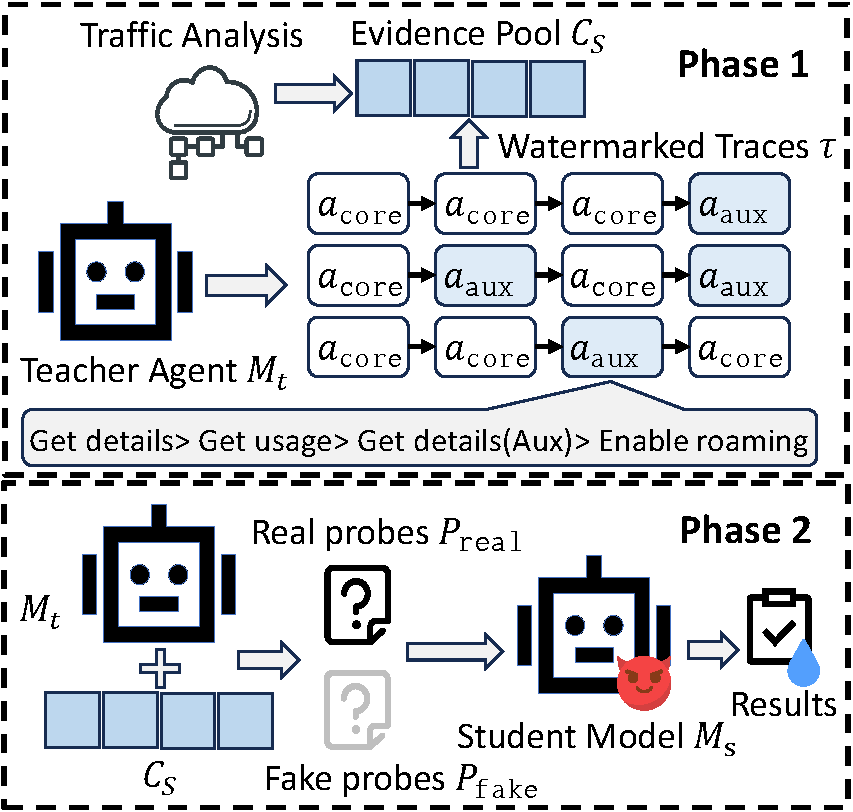
\includegraphics[width=0.85\columnwidth]{figure/overview.pdf}
\caption{Overview of \name{}. \textbf{Phase 1:} the owner embeds the watermark by inserting aux behaviors; \textbf{Phase 2:} the owner retrieves the private evidence to construct paired real and fake probes and verify a suspect student model. \textcolor[HTML]{BDD7EE}{\rule{0.85em}{0.85em}} denotes watermarked thing.}
\label{fig:overview}
\end{figure}

\subsection{Watermark Embedding Algorithm}

\label{sec:watermark_embedding}
Unlike previous watermarking methods that directly change the generated text or the teacher model's actions~\cite{wang2026protecting,an2026sequential}, \name{} embeds watermarks by adding extra, non-essential auxiliary actions into the agent's trajectory. By doing this, \name{} keeps the teacher model's performance high while creating strong evidence for later tracing. Also, to stay hidden, the added aux actions look and act exactly like normal tool calls: they use valid tools and bind strictly to normal parameter values derived from the interaction history. Based on the threat model described in Section \ref{sec:preliminaries}, the owner can subsequently identify suspicious traces from the API traffic and export their privately saved watermark evidence for later verification. The entire embedding process consists of three main stages shown in Figure\ref{fig:watermark_embedding_protocol}: safe tool classification, dynamic scheduling and candidate generation, and private evidence retention.

\partitle{Safe tool classification} To ensure aux actions will not change the environment state, \name{} applies a conservative safety policy to the tool schema $\mathcal{F}$ of trace $\tau$. Since the system operates as an agent-as-a-service~\cite{li2026aidev}, this safety evaluation is performed in advance and cached to avoid real-time latency. An offline safety model $\mathcal{M}_{\mathtt{safe}}$ evaluates the tool schema $\mathcal{F}$ and maps each tool $f \in \mathcal{F}$ to a safety label as shown in Eq.\ref{equ:safeclassfier}:
\begin{equation}
\mathcal{M}_{\mathtt{safe}}(f)=\begin{cases}\mathtt{safe},&\text{if }f\text{ is read-only,}\\\mathtt{unsafe},&\text{otherwise.}\end{cases}
\label{equ:safeclassfier}
\end{equation}
The system exclusively permits tools from the valid subset $\mathcal{F}_{\mathtt{safe}}=\{f \in \mathcal{F} \mid \mathcal{M}_{\mathtt{safe}}(f)=\mathtt{safe}\}$, categorically rejecting any action that changes the environment state or influences the task process.

\partitle{Dynamic scheduling} Having established the safe tool subset $\mathcal{F}_{\mathtt{safe}}$, the system must determine when to invoke these aux action during the interaction as the watermarking. To make watermark positions unpredictable, \name{} dynamically evaluates whether to inject an aux action at step $t$ immediately after the core action $a_{\mathtt{core}}^{t-1}$ finishes. If skipped, the system waits and checks again after the next core action. For each trajectory $\tau$ named as $\mathtt{id}_\tau$ of an account $a$, the system keeps a release probability $p_t$ and a remaining budget $b_t$ at step $t$. Immediately after the core action $a_{\mathtt{core}}^{t-1}$ finishes, the system uses a cryptographic hash function $\mathtt{Hash}(\cdot) \to [0,1)$~\cite{preneel1994cryptographic} parameterized by the owner's secret key $k$ to compute a uniformly distributed random value $u_t$, as defined in Eq.~\ref{equ:hash}:
\begin{equation}
    \label{equ:hash}
u_t = \operatorname{\mathtt{Hash}}(k \mathbin\Vert a \mathbin\Vert \mathtt{id}_\tau \mathbin\Vert t) \in [0, 1).
\end{equation}
The system tries to add an aux action when $b_t>0$ and $u_t<p_t$. Depending on whether the auxiliary action is successfully inserted or the turn is skipped (due to generation failure or unmet conditions), the system updates the trigger probability and remaining budget for the next turn as follows:
\begin{equation}
\label{equ:pb_update}
(p_{t+1}, b_{t+1}) = 
\begin{cases}
(p_0, b_t - 1), & \text{if successfully inserted,} \\
(\min\{p_t + \Delta p, p_{\mathtt{max}}\}, b_t), & \text{otherwise.}
\end{cases}
\end{equation}
\partitle{Aux action embedding} If the dynamic scheduling condition is met, \name{} proceeds to generate and select the optimal aux action. To obtain high quality insertions, the system queries $\mathcal{M}_t$ to propose up to $K$ candidates. Each candidate $j$ is formulated as a tuple of a thought and an action: $(t_{\mathtt{aux}}^j, a_{\mathtt{aux}}^j)$, where the action $a_{\mathtt{aux}}^j$ consists of a tool $f_{\mathtt{aux}}^j$ and its arguments $p_{\mathtt{aux}}^j$. To ensure that the injected action perfectly blends into the trajectory, \name{} enforces a validation mechanism. First, the chosen tool must belong to the safe subset $\mathcal{F}_{\mathtt{safe}}$. Second, to prevent model hallucinations and ensure contextual rationality, the arguments $p_{\mathtt{aux}}^j$ must be extracted from the context (such as the core action's observation or history). Consequently, \name{} categorically discards any candidate that uses an unapproved tool or hallucinates untraceable arguments.

For each candidate $j$ that passes the validation, \name{} employs a scoring model $\mathcal{M}_q$ to evaluate it across three dimensions: naturalness, logical consistency, and distillability. Specifically, $\mathcal{M}_q$ assigns a relevance score $s_{\mathtt{rel}}^j$ to ensure the injected action aligns naturally with the task. Additionally, a reliability score $s_{\mathtt{relb}}^j$ ensures the high quality of the thought. Crucially, to foster a stable behavioral habit that the student model can easily absorb during distillation, the system calculates a repeatability score $s_{\mathtt{rep}}^j$. This score is directly determined by $n_j$, which represents the number of times the candidate's specific tool pairing $(f_{\mathtt{core}}, f_{\mathtt{aux}}^j)$ has been successfully injected in the account's history. The final score $S_j$ for candidate $j$ is computed as a weighted sum:
\begin{equation}
    S_j = \alpha \cdot s_{\mathtt{rel}}^j + \beta \cdot s_{\mathtt{relb}}^j + \gamma \cdot s_{\mathtt{rep}}^j.
    \label{equ:score}
\end{equation}
where $\alpha$, $\beta$, $\gamma$, and the step-function mapping from repeat count $n_j$ to $s_{\mathtt{rep}}^j$ are detailed in Appendix~\ref{sec:experimental-details}. The system selects the candidate with the highest score as the best aux action $(t_{\mathtt{aux}}^{\mathtt{best}}, a_{\mathtt{aux}}^{\mathtt{best}})$, then injects this aux action, establishing a natural sequence:
\begin{equation}
    t_{\mathtt{core}}^{t-1} \;\rightarrow\; a_{\mathtt{core}}^{t-1} \;\rightarrow\; o_{\mathtt{core}}^{t-1} \;\rightarrow\; t_{\mathtt{aux}}^{\mathtt{best}} \;\rightarrow\; a_{\mathtt{aux}}^{\mathtt{best}} \;\rightarrow\; o_{\mathtt{aux}}^{\mathtt{best}}.
\end{equation}
Based on the generation result, the system updates its states. A successful generation applies the success update (Eq.~\ref{equ:pb_update}) and increases the repeat count $n_{\mathtt{best}}$ for this tool pairing. If the generation fails, the system skips the insertion, applies the failure update, moves to generate core action and waits for next chance. For future auditing, every successful insertion creates a private evidence card $c_t$. To securely record the exact context and execution details, this card stores the historical context $h$, the preceding core action and observation, and the injected auxiliary tool parameters. It is saved as a tuple and added to the trajectory's evidence set $\mathcal{C}_\tau$:
\begin{equation}
    c_t = (h, t_{\mathtt{core}}^{t-1}, a_{\mathtt{core}}^{t-1}, o_{\mathtt{core}}^{t-1}, f_{\mathtt{aux}}^{\mathtt{best}}, p_{\mathtt{aux}}^{\mathtt{best}}), \quad \mathcal{C}_\tau = \mathcal{C}_\tau \cup \{c_t\}.
    \label{equ:evidence}
\end{equation}
As mentioned in our threat model, the model owner uses signals like querying styles, IPs, and traffic patterns to identify a suspicious set $\mathcal{S}$~\cite{chiang2024chatbot, liu2026embarrassingly}. The owner then collects the evidence from these flagged traces to form a global verification pool $\mathcal{C}_{\mathcal{S}} = \bigcup_{\tau \in \mathcal{S}} \mathcal{C}_\tau$.


\subsection{Watermark Detection}

\label{Detection}
While the embedding phase injects an aux action into the teacher's trajectory, the detection phase verifies if a suspect model $M_s$ has learned this specific behavior pattern. To achieve this, \name{} uses paired probes built from the combined evidence pool $\mathcal{C}_{\mathcal{S}}$ for verification as shown in Figure~\ref{fig:watermark_detection_protocol}.



\partitle{Paired probe construction} To verify watermark retention, \name{} constructs paired probes for the combined evidence pool $\mathcal{C}_{\mathcal{S}}$. A probe is formally defined as a prompt-target tuple: given a history and a core action as the prompt, the suspect model $\mathcal{M}_s$ is expected to output a specific aux action. Specifically, based on each evidence card, we derive two types of probes: real probes and  fake probes. This paired design ensures that the model $\mathcal{M}_s$ has genuinely memorized the specific watermarked trace, rather than unconditionally outputting the target action.

For the real side construction of each card $c_i \in \mathcal{C}_S$, the system first locates the nearest core action. To ensure that the suspect model $M_s$ has learned the expected behavior, \name{} creates up to $N$ parameterized variants for this real side by modifying one argument of the original core action, the system prompts the teacher model $\mathcal{M}_t$ to synchronously generate a logically consistent core triplet $(t_{\mathtt{core}}^j, a_{\mathtt{core}}^j, o_{\mathtt{core}}^j)$ alongside the new downstream target aux arguments $p_{\mathtt{aux}}^j$. This process directly generates a set of real side probes $p_{\mathtt{real}}^i$ for the specific card $c_i$ as shown in Eq.\ref{equ:probe real}:
    
\begin{equation}
    \label{equ:probe real}
p_{\mathtt{real}}^i = \left\{ (h, t_{\mathtt{core}}^j, a_{\mathtt{core}}^j, o_{\mathtt{core}}^j),\ (f_{\mathtt{aux}}, p_{\mathtt{aux}}^j)  \right\}_{j=1}^{N_i}.
\end{equation}
$h$ is the historical context, and $f_{\mathtt{aux}}$ is the targeted aux tool. Finally, the system aggregates the real-side probes from all cards to form the global real probe set $\mathcal{P}_{\mathtt{real}} = \bigcup_{c_i \in \mathcal{C}_S} p_{\mathtt{real}}^i$.

To better contrast with the real probes $\mathcal{P}_{\mathtt{real}}$, obtain more definitive statistical results, \name{} constructs a set of fake probes based on the $\mathcal{P}_{\mathtt{real}}$. This verifies whether the aux action stems from memorization rather than natural context or random chance.For this fake side. However, it prompts the teacher model $\mathcal{M}_t$ to replace the core action with a semantically similar fake core behavior $(\hat{t}_{\mathtt{core}}^j, \hat{a}_{\mathtt{core}}^j,\hat{o}_{\mathtt{core}}^j)$ that achieves the identical goal. This process generates the fake probe set $p_{\mathtt{fake}}^i$ for card $c_i$, directly matching the variants in $p_{\mathtt{real}}^i$ as shown in Eq.\ref{probe fake}:
    
\begin{equation}
    \label{probe fake}
p_{\mathtt{fake}}^i = \left\{  (h, \hat{t}_{\mathtt{core}}^j, \hat{a}_{\mathtt{core}}^j, \hat{o}_{\mathtt{core}}^j),\ (f_{\mathtt{aux}}, p_{\mathtt{aux}}^j)  \right\}_{j=1}^{N_i}.
\end{equation}
Thus, the strict difference between the paired probes lies only in the core action. Similar to the real side, the fake probe set is defined as $\mathcal{P}_{\mathtt{fake}} = \bigcup_{c_i \in \mathcal{C}_S} p_{\mathtt{fake}}^i$.

\partitle{Card-level statistical test} After generating the paired probes, \name{} evaluates the suspect model $M_s$ using $(\mathcal{P}_{\mathtt{real}}, \mathcal{P}_{\mathtt{fake}})$ and performs a card-level statistical test which is discussed in Appendix~\ref{sec:statistical-test-discussion}. For the $j$-th probe pair of card $c_i$, the expected aux action is $f_{\mathtt{aux}}$ and arguments $p_{\mathtt{aux}}^j$. Let $(f_{\mathtt{out}}, p_{\mathtt{out}})$ be the tool call parsed from the output of $M_s$. For both the real and fake sides, \name{} computes the toolhit indicator $t_{i,j}$ and the strict fullhit indicator $h_{i,j} \in \{0, 1\}$:

\begin{equation}
t_{i,j} = \operatorname{\mathtt{Match}}(f_{\mathtt{out}}, f_{\mathtt{aux}}), \quad h_{i,j} = t_{i,j} \cdot \operatorname{\mathtt{Match}}(p_{\mathtt{out}}, p_{\mathtt{aux}}^j).
\label{eq:probe-score}
\end{equation}
where the function $\operatorname{\mathtt{Match}}(\cdot, \cdot) \to \{0, 1\}$ evaluates to $1$ if and only if there is exact structural and value equivalence between its two arguments, and $0$ otherwise. Because the $N_i$ paired variants derived from the same card $c_i$ share an identical core-to-aux dependency, they are not independent samples. Therefore, \name{} aggregates the scores at the card level to calculate the real-side hit rate $R_i^{\mathtt{real}}$, the fake-side hit rate $R_i^{\mathtt{fake}}$, and their difference $\Delta_i$ for each card $c_i$ as shown in Eq.\ref{eq:probe-rate}:
\begin{equation}
    R_i^{\mathtt{real}} = \frac{1}{N_i} \sum_{j=1}^{N_i} h_{i,j}^{\mathtt{real}},\qquad
R_i^{\mathtt{fake}} = \frac{1}{N_i} \sum_{j=1}^{N_i} h_{i,j}^{\mathtt{fake}},\qquad
\Delta_i = R_i^{\mathtt{real}} - R_i^{\mathtt{fake}}.
\label{eq:probe-rate}
\end{equation}
To evaluate the verification, we establish the null hypothesis $H_0$ and the alternative hypothesis $H_1$. $H_0$ posits that the suspect model $\mathcal{M}_s$ has not learned the watermarked habit; any correct action is due to general context or innate biases. Conversely, $H_1$ asserts that $\mathcal{M}_s$ has memorized the watermark, making it significantly more likely to output the target action on real probes. Based on the performance difference $\Delta_i$ for each card $c_i$, we classify the outcomes into a real win ($\Delta_i > 0$), a fake win ($\Delta_i < 0$), or a tie ($\Delta_i = 0$). Excluding ties, let $w$ and $\ell$ be the numbers of real and fake wins across $\mathcal{C}_{\mathcal{S}}$. The $p$-value is computed using a one-sided exact sign-test~\cite{hollander2013nonparametric}:

\begin{equation}
    p\mathtt{-value} = \sum_{k=w}^{w+\ell}\binom{w+\ell}{k}2^{-(w+\ell)}.
\end{equation}
where $p\mathtt{-value} = 1$ if $w+\ell=0$. To reject $H_0$ and declare a successful verification, \name{} requires dual criteria: the statistical significance must be $p\mathtt{-value} < p$, and the averaged real fullhit rate must exceed the fake rate by a predefined margin $r$ (i.e., $\frac{1}{|\mathcal{C}_{\mathcal{S}}|} \sum \Delta_i \geq r$). This empirical margin absorbs unpredictable fluctuations caused by context rewriting in the fake probes and guards against false positives. Appendix~\ref{sec:experimental-details} specifies the hyperparameters $p$, $r$, and $N$.


\subsection{Trace-Level Attribution} \label{subsec:trace_level}

While the detection protocol in Section~\ref{Detection} determines whether a suspect model $\mathcal{M}_s$ has distilled from $\mathcal{M}_t$, it cannot pinpoint which traces within $\mathcal{S}$ were utilized. For exact attribution, \name{} introduces a trace-level attribution. For each evaluated trace $\tau$, the system computes four rates to capture both exact and partial matches: the strict full-hit rates $R_\tau^{\mathtt{real}}$ and $R_\tau^{\mathtt{fake}}$, and the toolhit-only rates $T_\tau^{\mathtt{real}}$ and $T_\tau^{\mathtt{fake}}$ (where $t_{i,j}=1 \land h_{i,j}=0$). To ensure fair comparison across traces, \name{} normalizes each rate into an average-rank quantile $Q(\cdot) \in (0, 1)$:

\begin{equation}
    Q(x_\tau) = \frac{\operatorname{\mathtt{rank}}_{\mathtt{avg}}(x_\tau)}{|\mathcal{S}| + 1}.
\end{equation}
The attribution logic is designed as follows: $Q(R_\tau^{\mathtt{real}})$ acts as the primary positive signal for trace memorization. Conversely, if the model outputs the target aux action even on the fake probes, it implies innate biases rather than specific watermark retention. Thus, $Q(R_\tau^{\mathtt{fake}})$ serves as a penalty term. Furthermore, the toolhit-only terms address partial memorization, providing supplementary evidence to calibrate the final score. Consequently, \name{} ranks these traces using a score $S_\tau$:
    
\begin{equation}
    S_\tau = Q(R_\tau^{\mathtt{real}}) - \alpha' Q(R_\tau^{\mathtt{fake}}) + \beta' Q(T_\tau^{\mathtt{real}}) - \gamma' Q(T_\tau^{\mathtt{fake}}).
    \label{eq:trace-score}
\end{equation}
where the empirical weighting parameters $\alpha'$, $\beta'$, and $\gamma'$ are detailed in Appendix~\ref{sec:experimental-details}. Finally, the system identifies the top-$K$ traces with the highest $S_\tau$ most likely included in the training set $\mathcal{D}$.

